\documentclass[11pt,psfig]{article}
\usepackage{epsfig}
\usepackage{times}
\usepackage{amssymb}
\usepackage{float}

\newcount\refno\refno=1
\def\ref{\the\refno \global\advance\refno by 1}
\def\ux{\underline{x}}
\def\uw{\underline{w}}
\def\bw{\underline{w}}
\def\ut{\underline{\theta}}
\def\umu{\underline{\mu}} 
\def\bmu{\underline{\mu}} 
\def\be{p_e^*}
\newcount\eqnumber\eqnumber=1
\def\eq{\the \eqnumber \global\advance\eqnumber by 1}
\def\eqs{\eq}
\def\eqn{\eqno(\eq)}

 \pagestyle{empty}
\def\baselinestretch{1.1}
\topmargin1in \headsep0.3in
\topmargin0in \oddsidemargin0in \textwidth6.5in \textheight8.5in
\begin{document}
\setlength{\parskip}{1.2ex plus0.3ex minus 0.3ex}


\thispagestyle{empty} \pagestyle{myheadings} \markright{Homework
1: CS 273, Machine Learning: Winter 2015}



\title{CS 273 Homework 1}
\author{Zachary DeStefano, 15247592}
\date{Due Date: Tuesday, January 13, 2015}

\maketitle

\vfill\eject

%\begin{figure}[H]
%\centering
%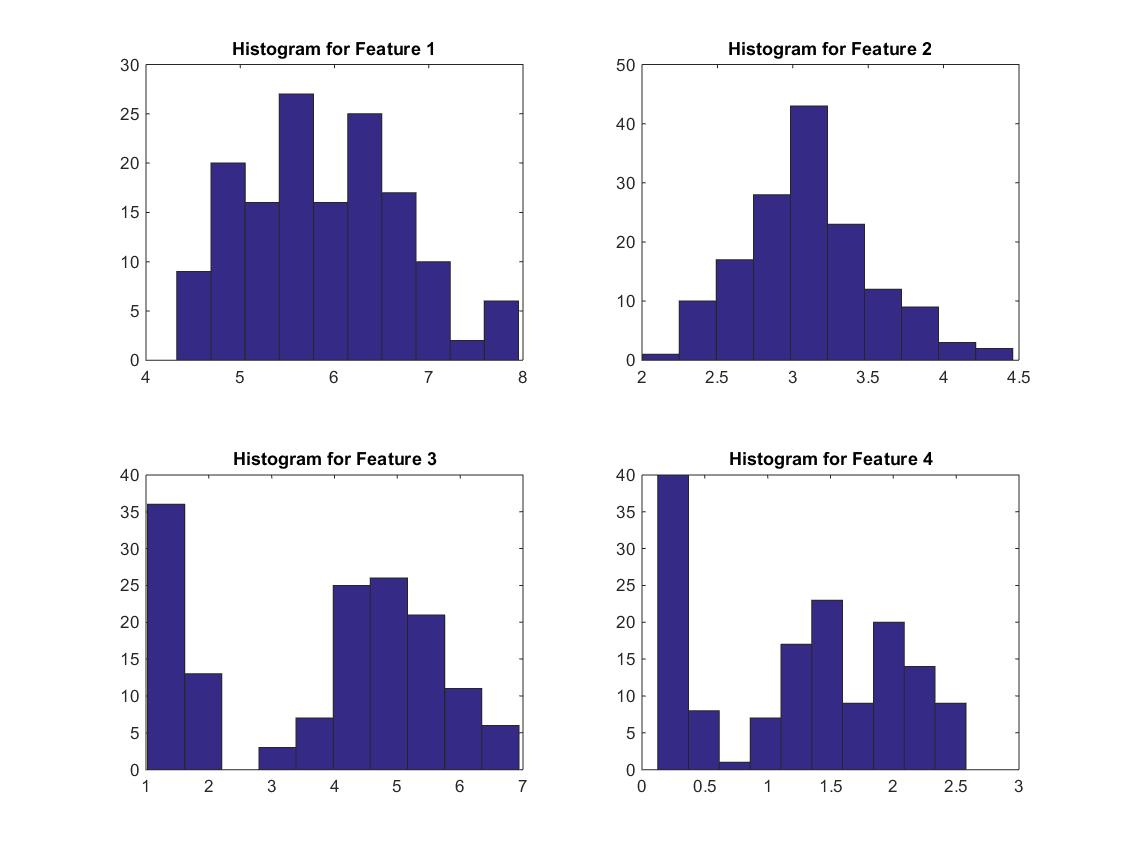
\includegraphics[width=\columnwidth]{prob1bHistograms.jpg}
%\caption{Histograms for each feature}
%\end{figure}

\section*{Problem 1}

\subsection*{Problem 1, Part a}

The number of features is 4\\
The number of observations is 148\\

\subsection*{Problem 1, Part b}

\begin{figure}[H]
\centering
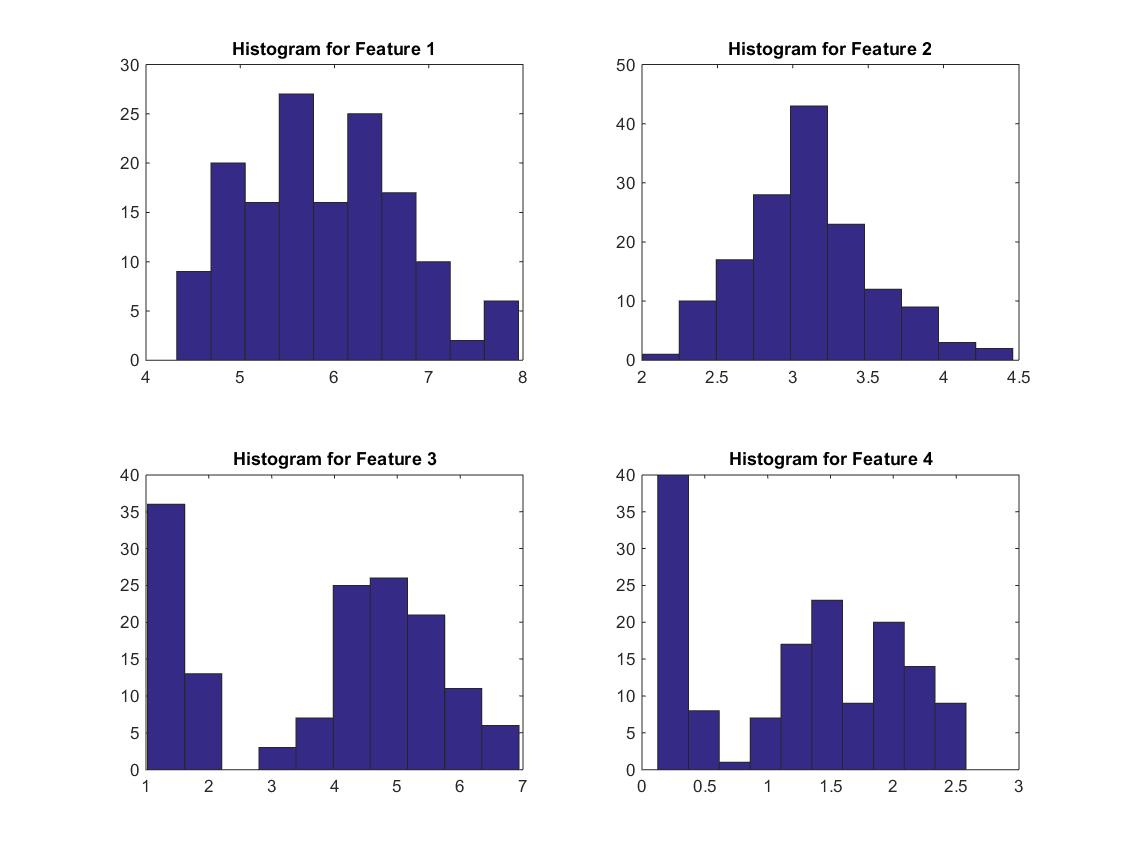
\includegraphics[width=\columnwidth]{prob1bHistograms.jpg}
\caption{Histograms for each feature}
\end{figure}

\newpage

\subsection*{Problem 1, Part c}

The mean of feature 1 is 5.9001\\
The mean of feature 2 is 3.0989\\
The mean of feature 3 is 3.8196\\
The mean of feature 4 is 1.2526\\

\subsection*{Problem 1, Part d}

The variance of feature 1 is 0.6993\\
The variance of feature 2 is 0.1916\\
The variance of feature 3 is 3.0976\\
The variance of feature 4 is 0.5797\\
\\
The standard deviation of feature 1 is 0.8362\\
The standard deviation of feature 2 is 0.4378\\
The standard deviation of feature 3 is 1.7600\\
The standard deviation of feature 4 is 0.7613\\

\subsection*{Problem 1, Part e}

Here is the code for part E. The initial parts of the code covers previous parts of this problem. 
\begin{verbatim}
iris = load('data/iris.txt');
y = iris(:,end);
X = iris(:,1:end-1);

%part A
numFeatures = size(X,2);
numDataPoints = size(X,1);

%put features into vectors
feature1 = X(:,1);
feature2 = X(:,2);
feature3 = X(:,3);
feature4 = X(:,4);

%part B
figure
subplot(2,2,1)
hist(feature1)
title('Histogram for Feature 1')
subplot(2,2,2)
hist(feature2)
title('Histogram for Feature 2')
subplot(2,2,3)
hist(feature3)
title('Histogram for Feature 3')
subplot(2,2,4)
hist(feature4)
title('Histogram for Feature 4')

%part C
mean1 = mean(feature1);
mean2 = mean(feature2);
mean3 = mean(feature3);
mean4 = mean(feature4);


%part D

%compute the variance
var1 = var(feature1);
var2 = var(feature2);
var3 = var(feature3);
var4 = var(feature4);

%compute the standard deviation
std1 = std(feature1);
std2 = std(feature2);
std3 = std(feature3);
std4 = std(feature4);

%part E
% Normalizes the data
normalize1 = (feature1-mean1)/std1;
normalize2 = (feature2-mean2)/std2;
normalize3 = (feature3-mean3)/std3;
normalize4 = (feature4-mean4)/std4;

\end{verbatim}

\subsection*{Problem 1, Part f}

\begin{figure}[H]
\centering
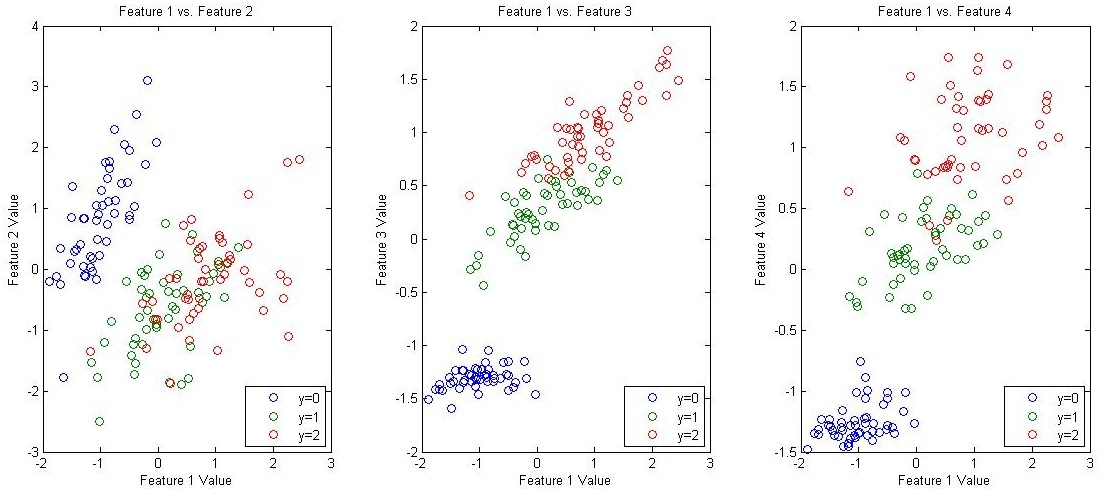
\includegraphics[width=\columnwidth]{prob1fScatterPlots.jpg}
\caption{The scatter plots for Problem 1f}
\end{figure}

This is the code to make those plots. It is a continuation of the code posted for part e. 
\begin{verbatim}
size = 30;
figure
subplot(1,3,1)
scatter(normalize1,normalize2,size,y);
title('Feature 1 vs. Feature 2');
xlabel('Feature 1 Value');
ylabel('Feature 2 Value');
subplot(1,3,2)
scatter(normalize1,normalize3,size,y);
title('Feature 1 vs. Feature 3');
xlabel('Feature 1 Value');
ylabel('Feature 3 Value');
subplot(1,3,3)
scatter(normalize1,normalize4,size,y);
title('Feature 1 vs. Feature 4');
xlabel('Feature 1 Value');
ylabel('Feature 4 Value');
\end{verbatim}

\newpage

\section*{Problem 2}

\subsection*{Problem 2, Part a}

These are the plots for part a

\begin{figure}[H]
\centering
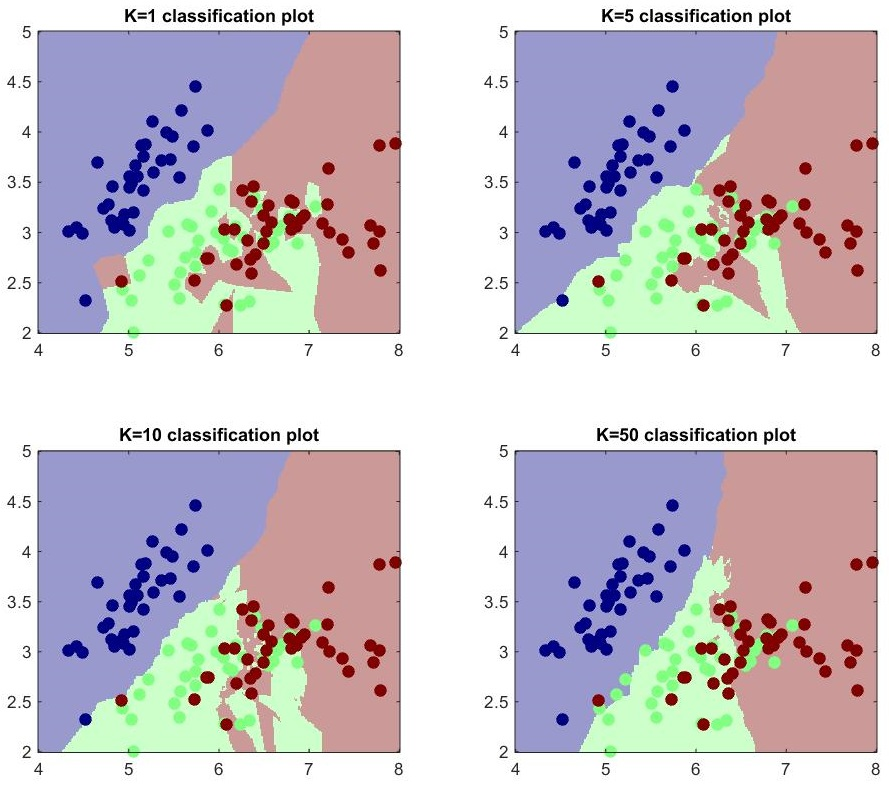
\includegraphics[width=\columnwidth]{prob2aPlots.jpg}
\caption{The scatter plots for Problem 2a}
\end{figure}

\newpage

Here is the code I used to generate those plots

\begin{verbatim}
%InitialPart
iris=load('data/iris.txt'); 
y=iris(:,end); 
X=iris(:,1:end-1);

[X y] = shuffleData(X,y); % shuffle data randomly
[Xtr Xte Ytr Yte] = splitData(X,y, .75); % split data into 75/25 train/test

%gets the first 2 features
XtrFirstTwo = Xtr(:,1:2);
XteFirstTwo = Xte(:,1:2);

%partA
figure
Kvals = [1,5,10,50];
for i=1:4
   K = Kvals(i);
   
   %train the classifier
   knn = knnClassify( XtrFirstTwo, Ytr, K );
   
   % make 2D classification plot
   subplot(2,2,i)
   plotClassify2D( knn, XtrFirstTwo, Ytr );
   title(strcat('K=',num2str(K),' classification plot'));
end
\end{verbatim}

\newpage

\subsection*{Problem 2, Part b}

Here is the training error (in Red) and the test error (in green) as the value of K increases. \\
Based on this plot, I would recommend $K=50$

\begin{figure}[H]
\centering
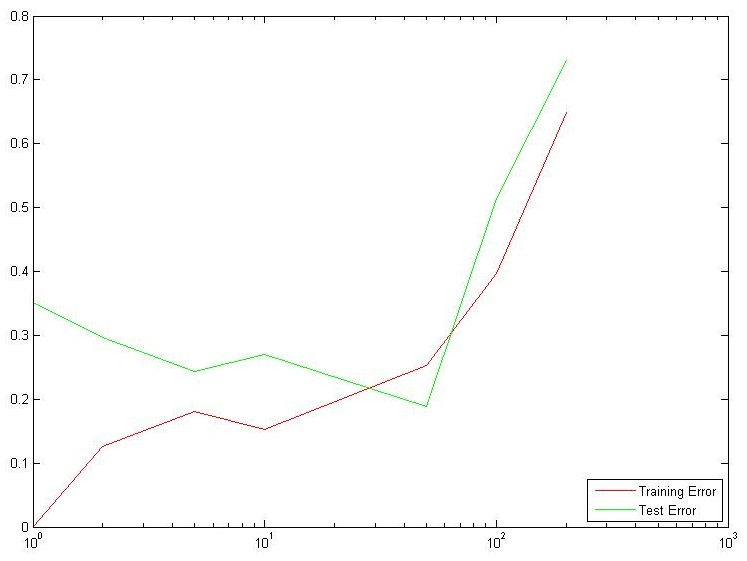
\includegraphics[width=\columnwidth]{prob2bPlot.jpg}
\caption{The semilog plot for Problem 2}
\end{figure}

\newpage

This is the rest of the code for problem 2, the part which was used to make the plots for part b. 

\begin{verbatim}
%part B
Kvals=[1,2,5,10,50,100,200];
errTrain=zeros(1,length(Kvals));
errTest = zeros(1,length(Kvals));
for i=1:length(Kvals)
    K = Kvals(i);
    learner = knnClassify( XtrFirstTwo, Ytr, K );
    YhatTr = predict(learner,XtrFirstTwo);
    errTrain(i)=length(find(YhatTr~=Ytr))/length(Ytr);
    
    YhatTe = predict(learner,XteFirstTwo);
    errTest(i)=length(find(YhatTe~=Yte))/length(Yte);
end;
figure
hold on
semilogx(Kvals,errTrain,'-','LineWidth',2,'Color','red');
semilogx(Kvals,errTest,'-','LineWidth',2,'Color','green');
hold off
\end{verbatim}

\end{document}








